\section{Parameter estimation and measurement models}
\label{sec:estimation}
% P:estimation-01
A parameter fit compares observations $y_k$ with model predictions $\hat y_k(\boldsymbol\theta)$ through the scaled least-squares objective
\begin{equation}
\min_{\boldsymbol\theta}\ \tfrac12\sum_k w_k r_k(\boldsymbol\theta)^2,
\qquad r_k=\frac{\hat y_k(\boldsymbol\theta)-y_k}{s_k}\quad\text{or}\quad r_k=\ln(\hat y_k/y_k),
\label{eq:fit}
\end{equation}
where $s_k>0$ is a numerical scale in the observation's units for a difference residual, and $w_k\geq0$ is a dimensionless relative weight.
The log-ratio residual is dimensionless, has no separate scale and requires positive predicted and observed values.
The active coordinates $\boldsymbol\theta$ are affine maps of physical parameters: residual equation-of-state parameters such as $k_{ij}$, segment diameters or association energies, a scalar $\ln K$ on a reaction's declared basis, and the coefficients $a$, $b$, $c$ and $d$ of Eq.~\eqref{eq:lnK}; reactions are identified by name rather than by position.
The package minimizes Eq.~\eqref{eq:fit} within declared bounds with the Levenberg--Marquardt trust-region method of the Ceres solver~\citep{agarwalCeresSolver2023}.
Every state is solved once per trial point, and a state that fails to solve is a failed evaluation, never a zero residual.

% P:estimation-02
Prediction derivatives of solved observations, $\partial\hat y_k/\partial\theta_j$, are assembled from Eq.~\eqref{eq:solved-actions} with $\mathbf{y}_\theta=-\mathbf{F}_\mathbf{y}^{-1}\mathbf{F}_\theta$ evaluated as a linear solve.
The optimizer Jacobian multiplies each prediction derivative by $\sqrt{w_k}/s_k$ for a difference residual or $\sqrt{w_k}/\hat y_k$ for a log-ratio residual.
A reaction-law coordinate enters $\mathbf{F}_\theta$ only through the chemical rows.
Supporting Information Table~\ref{tab:observations} lists the observations whose columns are verified, with their active coordinates and verified domain.
Observations also include pressure-specified density, source-basis $\ln K$, phase compositions and fractions, bubble pressures, and the enthalpy of a finite addition between two solved endpoints, including a solvent with exactly zero conserved carbon.
Reaction-reference declarations stay fixed during a fit.
Qualified finite-addition enthalpy observations admit referenced endpoints with solved temperature, using the reference and caloric derivatives at each endpoint's temperature.
Other observations retain their stated domain limits, and an available state-derivative order implies no higher fitting order.
A local parameter covariance is reported from the scaled Jacobian when the fit ends in the interior of the bounds with full rank, and is withheld at an active bound or under rank deficiency.

\subsection{Measurement errors, correlated data and local uncertainty}
% P:estimation-06
The numerical scales and relative weights in Eq.~\eqref{eq:fit} do not by themselves specify measurement uncertainty.
The implemented measurement-error model is Gaussian and uses difference residuals with declared physical standard deviations and unit relative weights for the included observations.
When physical input uncertainty is declared, standardized corrections to measured temperature, pressure or admitted feed coordinates join the model parameters as unknowns.
The objective includes both the corrected-output errors and one penalty per shared input measurement.
A declared known covariance matrix can couple errors across observations and inputs.
Writing the standardized error vector as $\mathbf{e}$ and its covariance as $\mathbf{C}=\mathbf{L}\mathbf{L}^{\mathsf T}$ gives
\begin{equation}
\mathbf{L}\mathbf{z}=\mathbf{e},\qquad
\min\tfrac12\|\mathbf{z}\|_2^2,\qquad
\mathbf{L}\mathbf{J}_{z}=\mathbf{J}_{e}.
\label{eq:whitening}
\end{equation}
The matrix is factored once after symmetry and positive-definiteness checks; it is neither repaired nor replaced by a pseudoinverse.
The same triangular solve transforms every complete Jacobian column, preserving the connection between the objective and its derivatives.
A failed physical state remains a failed trial after whitening.

% P:estimation-07
Parameter covariance is conditional on the supplied error model and a regular local linearization.
Uncertain-input directions are eliminated from the complete standardized Jacobian.
Active bounds, deficient rank or unfinished fitting withhold covariance; known absolute uncertainties supply no estimated common-variance multiplier.
Local rank and covariance do not establish global identifiability or predictive accuracy.


\subsection{Electrolyte observations and guarded minimax fitting}
% P:estimation-03
For electrolytes, the observations include mean ionic activity and osmotic coefficients, ion solvation Gibbs energies and relative permittivities.
A Born diameter can be held by a declared hydration Gibbs energy: an inner root solve then makes the diameter a dependent coordinate, and the implicit first derivative of that root enters every Jacobian column.
The least-squares covariance is then conditional on the fixed hydration targets.

% P:estimation-04
Guarded minimax estimation instead minimizes the largest absolute decadic target error $t$,
\begin{equation}
\min_{\boldsymbol\theta,t}\ t\qquad\text{subject to}\quad \lvert e_k(\boldsymbol\theta)\rvert\le t\ \ (k\in\mathcal{T}),\qquad g_m(\boldsymbol\theta)\le g_m^{\mathrm{base}}\ \ (m\in\mathcal{G}),
\label{eq:minimax}
\end{equation}
where $e_k=\log_{10}(\hat y_k/y_k)$ is the target error in decades and the guard functions $g_m$ constrain error measures for selected properties outside the target set $\mathcal{T}$ relative to a declared baseline.
Ipopt solves this epigraph problem with exact first derivatives of the target and guard errors, obtained from the prediction columns, and limited-memory curvature, unlike the exact-curvature equilibrium solves of Section~\ref{sec:driver}.
Several native starts, sharing one iteration and time budget, test for distinct local solutions.
If recomputed feasibility and first-order optimality checks pass, the result is a local stationary estimate of Eq.~\eqref{eq:minimax}; optimizer termination alone does not establish stationarity.
The estimate supplies no covariance or guarantee of global optimality or parameter identification.

% P:estimation-05
Manufactured parameter recovery and refined-difference observation columns test numerical correctness in Section~\ref{sec:verification}.
The physical fits below instead report calibration and separated prediction.




\subsection{Worked propane and chloride fits}
% P:estimation-08
Propane provides a short fit that can be followed from observations to prediction.
Saturation pressures and saturated-liquid mass densities measured by Glos et al.~\citep{Glos2004}, Table~2, supply three training temperatures: 210, 270 and 330~K.
The active physical parameters are dispersion energy, segment number and segment diameter; the objective uses six natural-log ratios with unit weights.
Listing~\ref{lst:fit} shows the observation part of that declaration.
These numerical weights do not use the measured expanded uncertainties, so a low objective does not imply statistical agreement within those uncertainties.

\begin{lstlisting}[language={},caption={Observation excerpt of the propane fit declaration; the active physical coordinates are dispersion energy, segment count and diameter.},label={lst:fit}]
"targets": ["saturation_pressure", "saturated_liquid_mass_density"],
"residuals": {"saturation_pressure": "log_ratio",
              "saturated_liquid_mass_density": "log_ratio"},
"multiplier": 1.0
\end{lstlisting}

% P:estimation-09
Four starts reach the same local solution within the precision that matters for the property comparison.
The fitted parameters are $\epsilon/k=208.51125$~K, $m=1.9964556$ and $\sigma=3.6194291$~\AA.
The fit is interior and its local Jacobian has full rank, which permits a conditional covariance but supplies no validated prediction interval.
Figure~\ref{fig:fits} marks the three training temperatures, 19 withheld temperatures and two stress temperatures, 110 and 340~K, at the ends of the measured range.
The withheld temperatures include 150~K, which the source baseline lists as a training state but this fit does not use.
On the withheld temperatures the fitted parameters give pressure and liquid-density average absolute relative deviations (AARDs) of 1.00\,\% and 0.180\,\%, against 1.07\,\% and 0.228\,\% for the published parameters; the two stress states give 22.0\,\% and 0.382\,\% after fitting.
The refit therefore mainly improves the liquid density; the withheld pressure deviation changes little.
These populations include extrapolation below the training range; no pooled accuracy is assigned to an arbitrary new temperature.

\begin{figure}[pos=p]
\centering
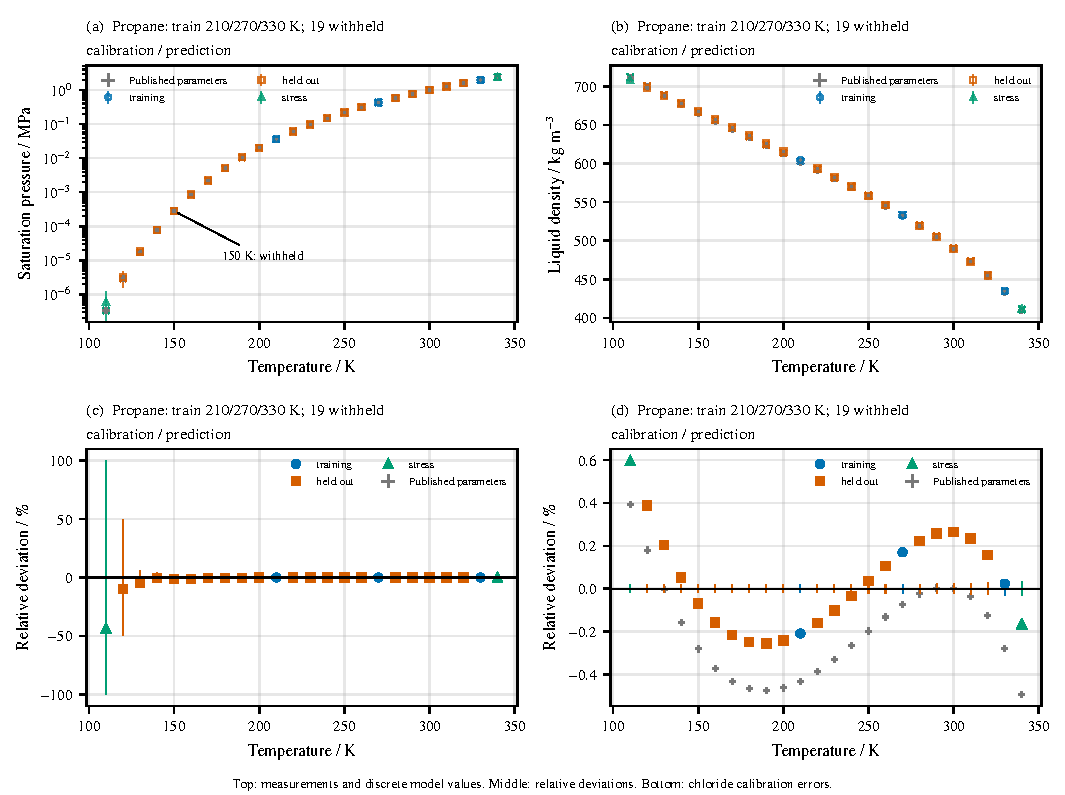
\includegraphics[width=0.91\linewidth,height=0.45\textheight,keepaspectratio]{F15-propane-fit}\par
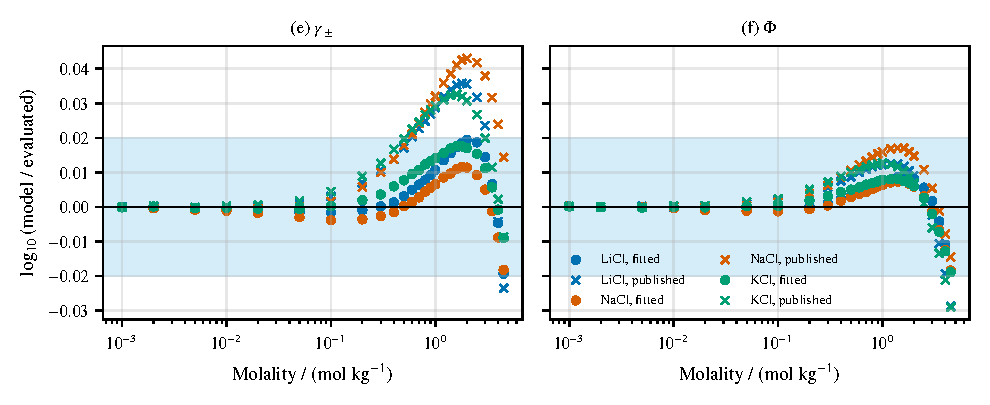
\includegraphics[width=0.91\linewidth,height=0.25\textheight,keepaspectratio]{chloride-calibration}
\caption{Calibration and transfer are separate parts of parameter estimation.
Top four panels: propane saturation pressure and liquid density against the measurements of Glos et al.\ after the three-temperature fit, with training, withheld and stress temperatures marked; in the deviation panels, bars are the expanded measurement uncertainties and grey crosses are the published parameters~\citep{Glos2004,Gross2001}.
Bottom: decadic errors $\log_{10}(\text{model}/\text{evaluated})$ of the mean ionic activity and osmotic coefficients of LiCl, NaCl and KCl at 298.15~K for the guarded minimax fit and the published parameters, with the $\pm0.02$ target band shaded~\citep{HamerWu1972,Figiel2025}.
The chloride data were fitted, so the bottom panels show calibration only.}
\label{fig:fits}
\end{figure}

% P:estimation-10
The electrolyte example uses a different objective for a different purpose.
Guarded minimax fits LiCl, NaCl and KCl activity and osmotic coefficients to the evaluated Hamer--Wu data~\citep{HamerWu1972}, Tables~9, 16 and~28, at 298.15~K and 100~kPa.
The 156 target quantities span 26 molalities per salt from 0.001 to 4.5~mol/kg.
Hydration targets hold Born diameters, and guards constrain bromide coefficients, transfer energies and aqueous permittivity relative to the published Figiel parameters~\citep{Figiel2025}.
The largest fitted target error is below 0.019371 decade, inside the declared 0.02-decade band; the published parameters exceed that band on 41 target rows.
A least-squares optimum also meets the target band but violates eight guard groups.
Thus the choice of estimator encodes which property deterioration is allowed, not merely which optimizer gives the smallest target sum.
Neither fit identifies unique electrolyte parameters or establishes independent mixture accuracy.
